\subsection{Steady-State Critical Flow Over an Uncertain Bed}

This test is designed to challenge the stochastic Galerkin model at representing highly non-Gaussian distributions of stochastic flow.
The uncertain bed elevation profile and inflow boundary condition are chosen in order to produce a nonlinear response such that the steady-state solution may be subcritical or transcritical depending on the hump amplitude.
Results of the stochastic Galerkin model are compared against a Monte Carlo simulation that serves as the reference solution.

The uncertain bed elevation is the smooth hump given by equation~\eqref{eqn:z-pc-coeffs}.
Subcritical boundary conditions are imposed such that the mean upstream discharge is \SI{1.65}{\meter\squared\per\second} and the mean downstream water elevation is \SI{1.5}{\meter}, with zero uncertainty on both upstream discharge and downstream water elevation.
These boundary conditions are chosen such that the flow is critical over the mean hump amplitude $\amean = \SI{0.6}{\meter}$ at $x = \SI{0}{\meter}$.
Since the hump amplitude is uncertain then the flow regime is also uncertain: if the hump amplitude is less than $\amean$ then the flow remains subcritical; if the hump amplitude is greater than $\amean$ then the flow regime becomes transcritical.

\begin{figure}
    \centering
    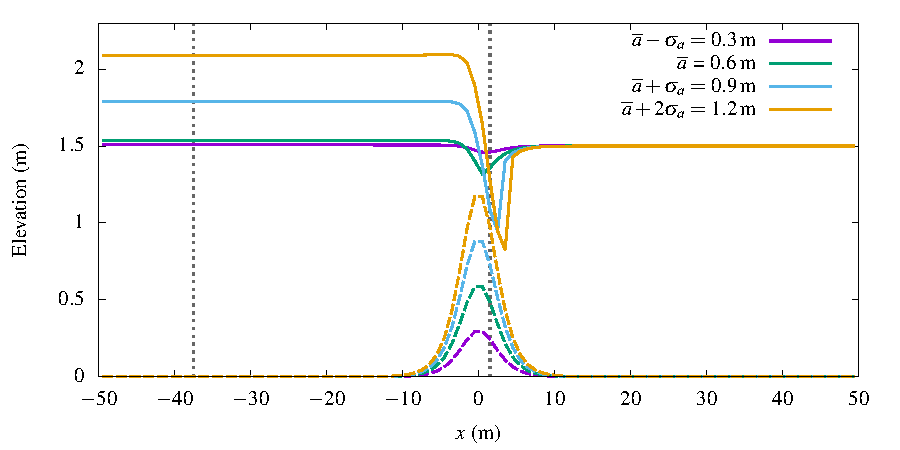
\includegraphics{fig-criticalSteadyState-examples.pdf}
    \caption{Well-balanced deterministic solutions using four hump amplitudes, $\amean - \sigma_a = \SI{0.3}{\meter}, \amean = \SI{0.6}{\meter}, \amean+\sigma_a = \SI{0.9}{\meter}$ and $\amean + 2\sigma_a = \SI{1.2}{\meter}$.
    Water elevation is shown with thick lines and the bed elevation profile is shown with thin lines.}
    \label{fig:criticalSteadyState-examples}
\end{figure}

To illustrate this behaviour, figure~\ref{fig:criticalSteadyState-examples} shows four deterministic solutions using different hump amplitudes.
Solutions from the well-balanced deterministic model are obtained at $t = \SI{500}{\second}$ when the water has converged on a steady state, with convergence measured by calculating the $\ell^2$ difference in water height between the current and previous timesteps.
By $t = \SI{500}{\second}$ all four deterministic solutions have converged down to $10^{-4}$.
For a small hump with amplitude $\amean - \sigma_a = \SI{0.3}{\meter}$, the flow remains subcritical.
A linear increase in hump amplitude produces a strongly nonlinear response in the steady-state water profile, as seen in figure~\ref{fig:criticalSteadyState-examples}, 
The upstream boundary condition allows the upstream water elevation to increase nonlinearly, and a transcritical shock develops that increases in amplitude and moves further downstream with larger hump amplitudes.
Downstream of the hump, the mean water elevation is \SI{1.5}{\meter} with zero uncertainty, with this profile having propagated upstream from the imposed downstream boundary.

The stochastic Galerkin model is evaluated by comparing results against a Monte Carlo simulation that serves as a reference solution.
For the Monte Carlo iterations, the topography is generated using a random hump amplitude drawn from the Gaussian distribution given by $(\amean, \sigma_a)$ and so the topography will always be smooth.
If instead the topography was generated using $(\zmean(x), \sigma_z(x))$ then the topography would not be smooth and many more iterations would be needed to sample the stochastic solution space.
The random hump amplitude $a$ is constrained such that $\SI{0}{\meter} \leq a \leq \SI{1.4}{\meter}$ to avoid negative water heights.
2000 Monte Carlo iterations are performed so that the mean and standard deviation of water height are both converged statistically.
Statistical convergence is determined qualitatively, with water height statistics measured at $x = \SI{1.5}{\meter}$ where the variance is large and the probability distribution is highly non-Gaussian.

\subsubsection{Stochastic Galerkin and Monte Carlo solutions}

\begin{figure}
    \centering
    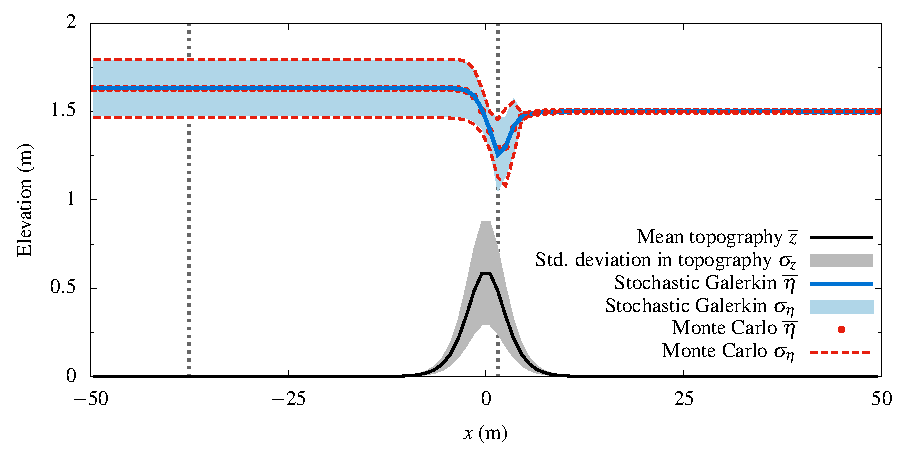
\includegraphics{fig-criticalSteadyState-flow.pdf}
    \caption{Solutions of steady state critical flow over an uncertain hump at $t = \SI{500}{\second}$, comparing stochastic Galerkin and Monte Carlo profiles of mean water elevation $\etamean$ and standard deviation in water elevation $\sigma_\eta$.
    Vertical dotted lines at $x = \SI{-37.5}{\meter}$ and $x = \SI{1.5}{\meter}$ mark the positions of the probability distributions shown in figure~\ref{fig:criticalSteadyState-pdf}.}
    \label{fig:criticalSteadyState-flow}
\end{figure}

In figure~\ref{fig:criticalSteadyState-flow}, spatial profiles of the water elevation statistics are obtained at $t = \SI{500}{\second}$ when the Monte Carlo iterations and stochastic Galerkin solution have converged down to $10^{-4}$.
The stochastic Galerkin model successfully represents the Monte Carlo reference profiles of the mean and standard deviation in water elevation.
Upstream of the hump, the stochastic Galerkin model produces a mean water elevation that is slightly too low, and a standard deviation that is slightly too small compared to the Monte Carlo reference solution.

The mean and standard deviation statistics are useful for summarising the spatial profile of uncertainty, but they are less meaningful for non-Gaussian probability distributions.
Since figure~\ref{fig:criticalSteadyState-examples} demonstrated that the response to an uncertain bed is strongly nonlinear then highly non-Gaussian probability distributions are expected.
Studying the probability distributions is particularly import for flood risk assessments that are concerned with extreme events that occur in the tails of the distributions.

Using the stochastic Galerkin method, the probability density function $f(u)$ for a stochastic variable $u$ can be calculated for a given element $i$ and time level $n$,
\begin{subequations}
\begin{align}
        f(u) = \sum_{k=1}^K \Mag{ \sum_{p=0}^P u_{i,p}^{(n)} \frac{\dee \Phi_p}{\dee \xi}(\randomroot_k)}^{-1} W(\randomroot_k)
%
\intertext{where $\randomroot_k$, $k=1, \ldots, K$ are the real roots of the polynomial}
%
        u - \sum_{p=0}^P u_{i,p}^{(n)} \Phi_p(\xi) = 0
\end{align}
\end{subequations}
which can be calculated numerically for a given value of $u$.

\begin{figure}
    \centering
    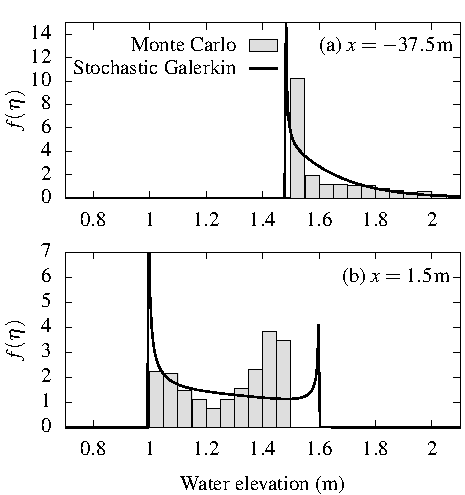
\includegraphics{fig-criticalSteadyState-pdf.pdf}
    \caption{Probability distributions of water elevation at (a) $x = \SI{-37.5}{\meter}$ and (b) $x = \SI{1.5}{\meter}$ for steady state critical flow over an uncertain hump at $t = \SI{500}{\second}$.}
    \label{fig:criticalSteadyState-pdf}
\end{figure}

Probability distributions are calculated at $t = \SI{500}{\second}$ at $x = \SI{-37.5}{\meter}$ and $x = \SI{1.5}{\meter}$.
The first point is far upstream of the hump where the water elevation is uncertain and spatially uniform.
The second point is immediately downstream of the hump in the region where transcritical shocks develop if the hump amplitude is sufficiently large.

%This test is designed to challenge stochastic Galerkin methods in representing a bimodal statistical distribution of water elevation
